\chapter{Related Work}
In this chapter we will introduce relevant publications regarding dental caries detection. We will focus mainly on detection from bitewing radiographs. Following that, methods for the segmentation of dental restorations will be briefly introduced.

\section{Dental caries detection}
Since 2017, more than ten publications have been regrading automatic caries detection from images \cite{PradosPrivado2020}. They differ in the way they approach caries localization and the types of images used. The following types of images have been used: Near-Infrared Transillumination images \cite{Casalegno2019,Schwendicke2020}, camera photographs \cite{Moutselos2019} and X-ray images, which may be further divided into bitewing X-ray images \cite{Moran2021, Cantu2020, Bayrakdar2021, Mao2021, Srivastava2017} panoramic X-ray images \cite{Lian2021} and periapical X-ray images \cite{Lee2018}.

All the related publications can be divided based on their approach to caries localization into three groups: Manual detection and classification, dental caries segmentation, and dental caries detection.

\subsection{Manuall detection and classification}
This section will in short introduce publications that approached caries detection in the following manner: First, they crop individual teeth from the X-ray image. Manual cropping or non-machine learning computer vision techniques were used for this purpose. After a tooth is extracted from the image, it is labeled by a professional. A classifier is trained on those image patches to decide if it contains a carious lesion.
\begin{itemize}
    \item First attempts to use a neural network for caries detection date back to 2008, when Kuang et al. \cite{Kuang2008} proposed an approach based on passing a patch from an image to a classifier, which decided if the patch contains caries or healthy enamel. Even though the performance of the proposed neural network was surpassed by 6.72\% by kernel SVM, it was still able to outperform an ordinary dentist by more than 5\% and was only 6\% worse than an experienced one
    \item Moran et al.\cite{Moran2021} used methods such as histogram equalization, Otsu's thresholding, and morphological operations to extract individual teeth from bitewing images. The dataset was labeled after teeth extraction by assigning one of three categories to each tooth. The categories were: Normal teeth, incipient lesions, and advanced lesions. A total of 112 radiographs have been processed this way resulting in 480 teeth with corresponding annotations. ResNet and Inception model was trained to perform the classification task, and the best-achieved accuracy was 73.3\% \cite{Moran2021}.
    \item{Mao at al. \cite{Mao2021}} did a similar preprocessing approach as Moran, only this time extracting unilateral teeth images instead of the whole teeth. A total of 3716 images of unilateral teeth were obtained. For the purpose of classification, AlexNet was used and got 90.3\% accuracy.
    \item{Lee et al. \cite{Lee2018}} published a similar approach with periapical images. The dataset with 3000 images was created manually by cropping out teeth from the X-ray image, keeping only those without bigger dental restorations. By the same process, two teeth at once were cropped from the image as well. After obtaining this dataset, GoogLeNet and Inception v3 architecture classifiers were trained, obtaining an accuracy of 89\%  for molars and 82\% for images with both premolars and molars.
\end{itemize}


\subsection{Dental caries segmentation}
There are publications where the authors approached the task of caries localization as a semantic segmentation. The advantage of this approach is the pixel precision of the lesion detection. On the other hand creation of a similar dataset is very time-consuming. An example of a dataset annotated in a pixel-wise manner can be seen in figure \ref{fig:segmentation_lit} as well as predictions of a model proposed by Cantu \cite{Cantu2020}.

\begin{figure}
    \centering
    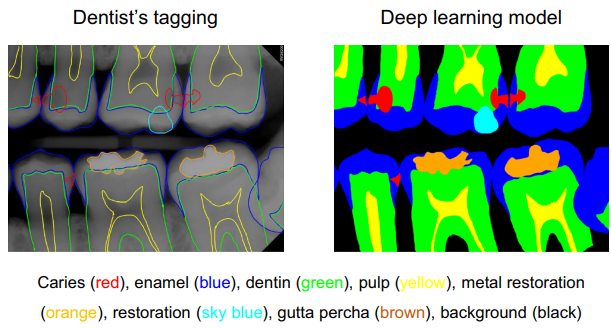
\includegraphics[width=\linewidth]{images/segmentation_bitewing_rich.png}
    \caption{Annotated bitewing radigraph and the same image post-processed, source \cite{Lee2021}}
    \label{fig:bitewing_dense}
\end{figure}

\begin{itemize}
    \item{Cantu et al. \cite{Cantu2020}} created dataset of 3686 bitewing images. A polygonal-shaped box was drawn over the caries independently by three dentists in each image. In the case of a unanimous decision, the annotation was kept in the dataset. Otherwise, the fourth dentist reviewed the annotation and decided if it should be kept or deleted. Cantu et al. used the U-Net model with EfficientNet B5 as a backbone. The model was evaluated per pixel, and its performance was compared against seven dentists, outperforming their mean performance in every metric.
    \item{Lian et al. \cite{Lian2021}} had the same approach as Cantu, but on panoramic images. In comparison with Cantu, following the segmentation, they cropped the region of interest around the segmented lesion and classified caries into one of four categories as described in the section. They achieved an IOU score of 0.785 on the segmentation task. In comparison, the best performing dentist achieved an IOU of 0.717. In the classification task, the model outperformed the mean dentist's performance.
    \item {Lee at al. \cite{Lee2021}}  approached the problem uniquely. In the dataset, consisting of 304 bitewing radiographs, they densely annotated each image by rectangles, denoting the position of dental caries and enamel, dentine, pulp, and gutta-percha restorations as well. The result of this annotation can be seen in image \ref{fig:bitewing_dense}. They used two independent U-net models to predict the position of dental caries and remaining structures in the image. The output of both models was post-processed and merged together. Even though, the model achieved an F1 score of 0.641, which is low compared to other publications. Predictions of the model helped dentists to improve their sensitivity ratio by 7 - 10\%.
\end{itemize}

\begin{figure}
    \centering
    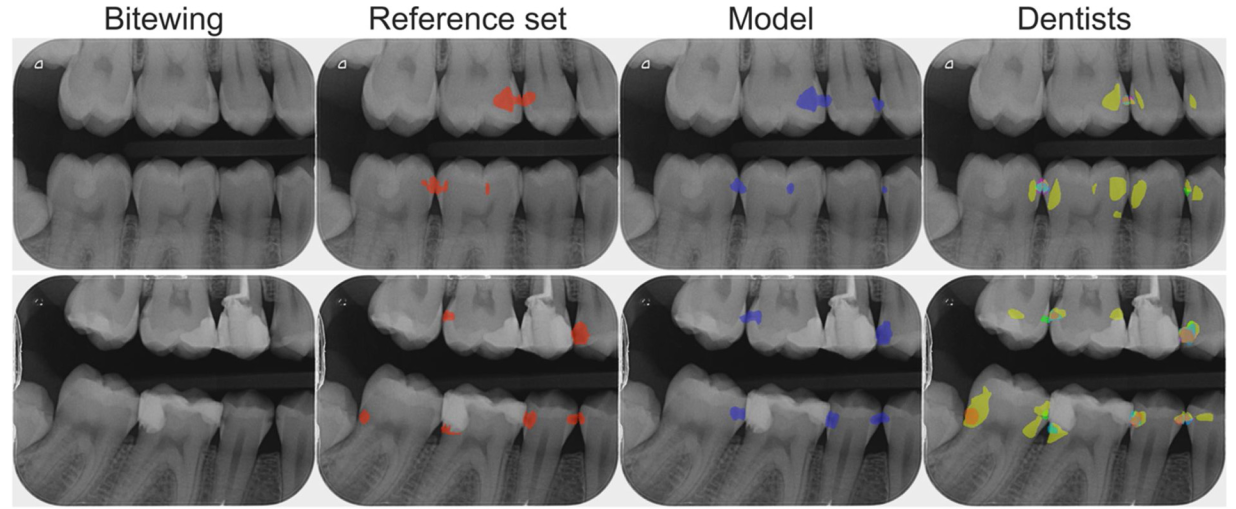
\includegraphics[width=\linewidth]{images/segmentatic_literature.png}
    \caption{Sample of data and predictions of model by }
    \label{fig:segmentation_lit}
\end{figure}

\subsection{Dental caries detection}
\begin{figure}
    \centering
    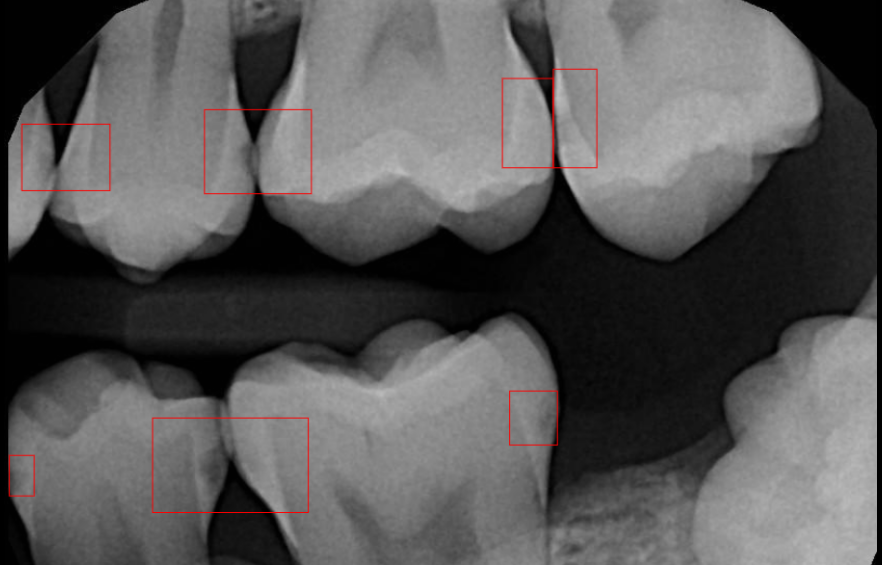
\includegraphics[width=\linewidth]{images/sirvastava_pred.png}
    \caption{Predictions of model proposed by Srivastava et al., source \cite{Srivastava2017}}
    \label{fig:srivastava_preds}
\end{figure}
\begin{itemize}
    \item{Srivastava et al. \cite{Srivastava2017}} trained a fully convolutional neural network with over 100 layers on a dataset containing more than 3000 bitewing radiographs. Position of tooth decay was denoted in pixel-wise manner. Even though the model predicts output masks in semantic segmantation fashion, the output is post-processed by fitting minimal bounding rectangle around the prediction as can be seen in figure \ref{fig:srivastava_preds}. After that the model is evaluated by computing IOU of the rectnagle with ground truth polygon, if the IOU is greater than 0.8, the detection is considered to be positive. Srivastava et al. claim, that their model outperforms each of three dentists included in the study by a big margin. Detailed results are in table \ref{tab:srivastava_results}.

          \begin{table}
              \centering
              \begin{tabular}{c||c|c|c|c|c}
                  Metric    & Model \cite{Srivastava2017} & Model \cite{Kumar2018} & Dr. 1 & Dr. 2 & Dr. 3 \\ \hline
                  Recall    & 0.805                       & 0.70                   & 0.477 & 0.433 & 0.344 \\ \hline
                  Precision & 0.615                       & 0.53                   & 0.63  & 0.815 & 0.891 \\ \hline
                  F1-Score  & 0.70                        & 0.614                  & 0.54  & 0.56  & 0.50
              \end{tabular}
              \caption{Results of models proposed in \cite{Srivastava2017} and \cite{Kumar2018}, compared with three dentists , modified}
              \label{tab:srivastava_results}
          \end{table}

    \item{The same author and Kumar \cite{Kumar2018}} published another paper, where they changed the model to U-Net, which was trained on an extended dataset of 6000 bitewing X-ray images. Hard example mining approach was tested by the authors but led to a decrease in performance. Even though U-Net architecture usually achieves better results on publicly available benchmarks \cite{paperwithcode, Zhang2019}, and the size of the dataset increased twofold, the performance of the model dropped by 15\%, see table \ref{tab:srivastava_results}. There is no information available about the evaluation protocol used by Kumar \cite{Kumar2018}, nor about the IOU threshold needed to consider a prediction to be correct. This makes it hard to estimate the cause of the performance drop.
    \item{Barakdar et al. \cite{Bayrakdar2021}} did both semantic segmentation and object detection. A dataset of 621 bitewing images was available for both of those tasks. They claim to use U-net for segmentation and VGGNet for object detection. In the paper, it is not mentioned how the VGGNet architecture for object classification was modified to perform an object detection task. The results of object detection were evaluated against five professionals in dentistry with different years of experience. The model has outperformed two dentists with 2 and 3 years of experience while being outperformed by a significant margin by all three dentists with 10 years of experience. The reported precision of the model is $0.78$, recall=$0.77$ and F1 score of $0.78$. The paper has no information about the overlap used to consider predictions to be correct. We assume it was set to be $0.5$.
    \item{Bayraktar2021 er al. \cite{Bayraktar2021}} solved only the object detection task on a dataset of 1000 bitewing images labeled by two experts with more than ten years of experience. With YOLOv3 architecture model, they achieved $AP@.5 = 0.872$ .
\end{itemize}

\section{Dental restorations detection}
To the author's knowledge, there are no available publications regrading the segmentation of dental restorations in bitewing radiographs. Therefore, we will introduce two methods that segment dental caries from panoramic X-ray images. Figures \ref{fig:restoration_seg_pub1}, \ref{fig:restoration_seg_pub2} contains samples of images used for restorations segmentation.
In addition two publications, where restoration detection was minor part of the work, will be mentioned.
\begin{figure}
    \begin{floatrow}[2]
        \ffigbox[1.25\FBwidth]{\caption{Results of segmentation algorithm proposed by Yeshua et al.\cite{Yeshua2019}}\label{fig:restoration_seg_pub1}}%
        {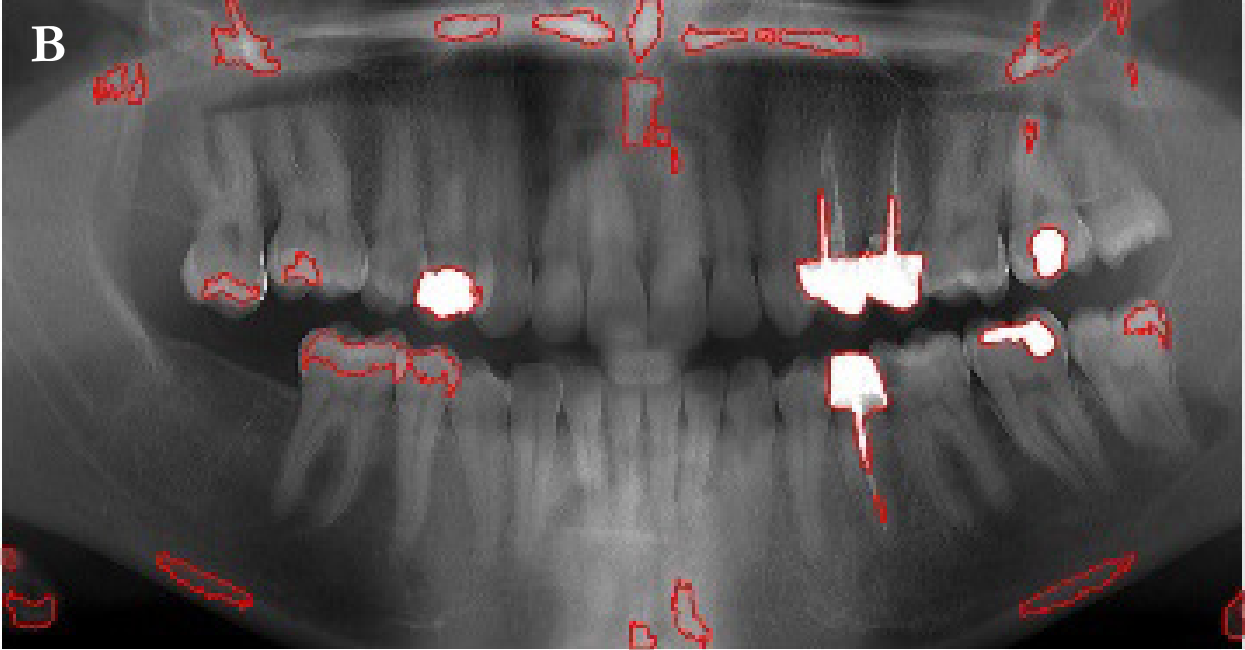
\includegraphics[width=\linewidth]{images/segmentation_opg.png}}\;
        \ffigbox[0.75\FBwidth]{\caption{Cropped region from panoramatic image with multiple restorations, source \cite{AbdallaAslan2020}}\label{fig:restoration_seg_pub2}}%
        {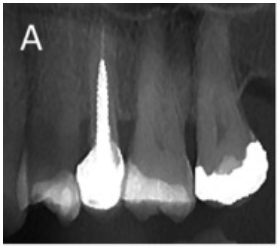
\includegraphics[width=\linewidth]{images/segmentation_crop.png}}
    \end{floatrow}
\end{figure}
\begin{itemize}
    \item{Mao et al. \cite{Mao2021}} classified dental segmentations in previously extracted image patches with unilateral teeth.
    \item{Lee at al. \cite{Lee2021}} did not focus directly on segmentation of restorations, but it was one of the classes semgented-out by their U-net architecture. There are no metrics available regarding the performance of the algorithm on dental restorations.
    \item{Abdalla-Aslan et al. \cite{AbdallaAslan2020}} used methods of classical computer vision to segment out restorations in panoramatic images. Their pipeline consisted of: Adaptive gaussian thresholding, morphological operations and deleting regions in peripheral areas of the image. The final algorithm had the precision and sensitivity of 0.33 and 0.946 respectively. After a successful detection, the restoration was classified into classes such as: dental implant, crown, amalgam filing, etc.
    \item {Yeshua et al. \cite{Yeshua2019}} solved the same problem as Abdalla-Aslan. Even the approach was more-less the same, but their solution achieved a precision of 0.568. They classified detected areas similarly to Abdalla-Aslan, having an extra category for false detections. After the removal of false detections, the precision was boosted to 0.98.
\end{itemize}